\section{Forca}

\begin{frame}
	\begin{block}{Jogo: Forca}
		\begin{itemize}
			\item O jogo forca é muito simples, uma pessoa escolhe uma palavra aleatória e escreve em um papel. Em seguida é desenhada uma linha tracejada, em outra folha de papel, onde cada traço representa uma letra da palavra escrita.
			
			\item Outra pessoa deve descobrir qual é foi a palavra escrita chutando letras. Cada letra certa a primeira pessoa deve escrever a letra em cima do tracejado de sua posição correspondente.
			
			\item Para as letras erradas será desenhada uma parte de um boneco (representando um ser humano, como pernas, braços cabeça e tronco) em um equipamento de morte da idade média denominado: Forca.
		\end{itemize}
	\end{block}
\end{frame}

\begin{frame}
	\begin{block}{Jogo: Forca}
		\begin{itemize}
			\item Exemplo de jogo: "forca"
		\end{itemize}
		\begin{figure}[!htb]
			\centering	  				
			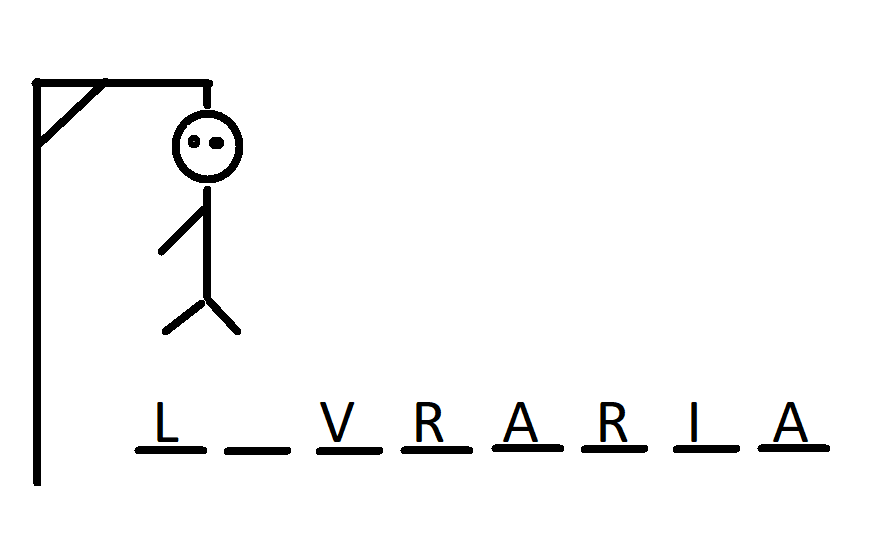
\includegraphics[height=3cm, width = 9cm]{./pic/forca.png}
			\caption{Jogo da forca \cite{Demonstre}}
			\label{fig_LLS_one}
		\end{figure}
	\end{block}
\end{frame}

\begin{frame}
	\begin{block}{Jogo: Forca}
		\begin{itemize}
			\item Nosso game vai precisar de um objeto palavra

			\item Nossa game vai precisar de um objeto Lista de palavras
		
			\item Nosso game precisa de condições de vitória, perda e continue jogando
		
			\item Nossa interface gráfica será o console
		\end{itemize}
	\end{block}
\end{frame}

\begin{frame}
	\begin{block}{Jogo: Forca}
		\begin{itemize}
			\item Mostrar o código para os alunos e explicar, mandar eles entenderem o código e produzirem um relatório sobre as partes do código.
		\end{itemize}
	\end{block}
\end{frame}